\documentclass{xduugthesis}

\usepackage{float} % \begin{figure}[H] 图片紧随文字
\usepackage{booktabs}
\usepackage{graphicx}
\usepackage{longtable}
% \usepackage{svg}
\usepackage{xcolor}
\usepackage{tabularray}
\usepackage{titlesec}

\titleformat{\subsection}
{\normalfont\zihao{4}\centering}
{\thesubsection}
{1em}
{}

\xdusetup{
style = { 
    cjk-font = fandol, 
    latin-font = tac,
    bib-backend = biblatex % -> biber
},
info = {
    title = {农业果实称重云端软件的设计与实现},
    department = {计算机科学与技术学院},
    major = {计算机科学与技术},
    author = {江志航},
    supervisor = {霍秋艳},
    class-id = {2103018},
    student-id = {20009100359},
    abstract = {abs_zh.tex},
    abstract* = {abs_en.tex},
    keywords = {智慧农业, 物联网, Spring Boot, Vue, YOLO},
    keywords* = {Smart Agriculture, IoT, Spring Boot, Vue, YOLO},
    bib-resource = {reference.bib},
    acknowledgements = {ack.tex}
}
}

% 之后注释掉
% \fancypagestyle{plain}{\pagestyle{fancy}\fancyhf{}\fancyhead[CO]{\rmfamily\zihao{5}\leftmark}\fancyfoot[LE]{\rmfamily\zihao{-5}\thepage}\fancyfoot[RO]{\rmfamily\zihao{-5}\thepage}\renewcommand{\headrulewidth}{0.75pt}}


\begin{document}

\chapter{绪论}

\section{选题背景与意义}

在全球人口持续增长以及人们对农产品品质与安全关注度日益提升的大背景下,农业的发展面临着前所未有的挑战与机遇。智慧农业作为一种融合了现代信息技术、生物技术、工程技术等多学科技术的新型农业发展模式\cite{赵春江2021智慧农业的发展现状与未来展望},正逐渐成为推动农业现代化进程的关键力量。它通过对农业生产过程中的各种数据进行实时采集、传输、分析和处理,实现了农业生产的精准化、智能化和自动化管理\cite{李道亮2012物联网与智慧农业},有效提高了农业生产效率、降低了生产成本、保障了农产品质量安全,为解决当前农业发展面临的诸多问题提供了新的思路和方法。

果实称重作为精准农业的重要环节,对于农业生产管理和决策具有不可或缺的作用\cite{罗锡文2016信息技术提升农业机械化水平}。首先,果实称重得到的数据能够为农民提供有关农作物产量的精确信息,帮助他们及时了解农作物的生长状况\cite{翁杨2019基于深度学习的农业植物表型研究综述},进而合理安排农事活动,如施肥、灌溉、病虫害防治等,以提高农作物的产量和质量。其次,通过对果实称重数据进行分析,还可以为农产品的市场定价、销售策略制定以及供应链管理提供有力的数据支持,有助于优化农产品的流通环节,提高农业经济效益\cite{Lipcsei2021AnalysisOA}。此外,在水果采摘环节,精确的称重能够实现水果按重量分级,满足不同消费者的需求,提升水果的市场竞争力\cite{Ji2019}。

然而,传统的果实称重主要依赖人工操作,存在着诸多明显的不足。首先,人工称重需要耗费大量的人力和时间,尤其是在果实收获季节,繁重的称重工作往往使人力成本大幅增加\cite{Jiang2012};其次,由于操作人员的疲劳、疏忽以及读数误差等因素的存在,人工称重获取的数据准确性和可靠性往往难以保证,并因此影响到后续的生产决策\cite{Chen2002};此外,人工称重的方式在数据记录和管理上也较为繁琐,难以实现数据的实时共享和高效分析,无法满足现代精准农业对数据快速处理和深度挖掘的需求\cite{Widagdo2020RecordingSO}。

随着云计算、边缘计算、图像识别等信息技术的飞速发展,将这些先进技术应用于农业领域,成为推动农业自动化和数字化转型的必然趋势。其一,云计算技术能够实现果实称重数据的实时采集、传输和存储,打破了时间和空间的限制,使得农民和农业管理者可以随时随地获取和管理称重数据\cite{李道亮2012物联网与智慧农业}。通过对海量称重数据的分析挖掘,云端软件能够为农业生产提供更加科学、精准的决策支持,如产量预测、市场趋势分析等,有助于农业生产者更好地应对市场变化,降低生产风险\cite{韩佳伟2022装备与信息协同促进现代智慧农业发展研究};其二,边缘计算技术能够实现在边端完成协议转换、信息认证、数据预处理等操作,不仅降低了延迟,也实现了在网络受限情况下称重活动的正常进行\cite{李娜2023基于云边协同计算的粉料仓自称重系统的设计与实现};其三,图像识别技术的应用让果实信息的处理实现自动化,果实的类别只需由云端自动完成识别,无需人工处理,让称重的效率大大提升\cite{Ni2024}。最后,云端软件可与其他农业信息化软件进行集成\cite{刘洋2013基于物联网与云计算服务的农业温室智能化平台研究与应用术},实现农业生产全过程的信息化管理,进一步提升农业生产的智能化水平,推动智慧农业的发展。

基于以上背景,本文研究将深入调研农业生产活动,归纳与分析具体需求,利用云计算、边缘计算、图像识别等软件技术,设计并开发农业果实称重云端软件,实现智能化的农业数据处理、高效的信息管理以及数据的可视化,为智慧农场的果实采摘称重管理提供了一个高效、稳定且功能丰富的解决方案,有助于推动智慧农场的精准收获和数字化管理。 

\section{国内外现状分析}

国外的智慧农业发展起步较早,农业果实称重技术与云端软件的应用研究取得了较为显著的成果。美国作为农业科技强国,在农业领域广泛应用了先进的传感器技术和物联网技术以提高生产效率\cite{赵春江2021智慧农业的发展现状与未来展望}。例如,一些大型农场采用了高精度的电子称重传感器,能够实时采集果实的重量数据,并通过无线传输技术将数据发送至云端服务器\cite{陈学庚2020农业机械与信息技术融合发展现状与方向}。在加利福尼亚州的部分果园,利用智能称重设备与云端软件相结合,实现了对水果采摘过程的精准监控和管理\cite{Ampatzidis2011}。农场主可以通过手机或电脑随时随地查看每个采摘区域的果实产量、重量分布等信息,从而及时调整采摘计划和资源分配。此外,美国还研发出基于图像识别和深度学习的果实称重与分级软件,通过对果实图像的分析\cite{Anisha2019FruitRU},不仅能够准确获取果实的重量,还能对果实的品质进行评估,进一步提高了果实称重与分级的智能化水平。

欧洲在农业果实称重云端软件的研究和应用方面同样处于领先地位。德国的一些农业企业开发了集成化的农业生产管理平台,其中包含了果实称重与数据分析模块\cite{Yin2020}。这些平台通过与各种农业设备的连接,实现了果实称重数据的自动采集和实时上传。同时,平台通过大数据分析技术对数据进行深度挖掘,为农业生产提供了全面的决策支持,如预测产量、优化种植方案等\cite{Phate2021}。荷兰则专注于温室农业中的果实称重技术研究,通过在温室中安装传感器网络,实现了对温室作物果实生长过程的全程监测和重量测量\cite{Graaf2004}。为了实现对温室作物的精准种植和高效管理,荷兰一些企业同样利用了云端软件对数据进行分析管理。

随着国内智慧农业的快速发展,农业果实称重云端软件的研究和应用也逐渐受到重视。近年来,国内高校和科技公司在该领域开展了大量的研究工作,并取得了一系列的成果。一些高校的研究团队开发了基于物联网的果实称重软件,通过将电子秤与物联网模块相结合,实现了果实称重数据的无线传输和远程监控\cite{Zhu2013}。并且山东的部分果园已经率先应用了这种物联网称重系统。通过该系统,果农可以在手机 APP 实时查看果实的称重数据,方便了果实采摘和销售管理\cite{Gao2023}。国内企业也积极投入到农业果实称重云端软件的研发和推广中。一些科技公司推出了针对不同农业场景的果实称重解决方案\cite{Ningbo2019},不仅提供了硬件设备,还开发了相应的软件平台,实现了数据的云端存储、分析和可视化展示,帮助农业生产者更好地管理果实称重数据,提高农业生产效率。

然而,目前的果实称重软件仍存在一些不足之处。一方面,部分果实称重软件的精度和稳定性有待提高,在复杂的农业生产环境中,容易受到温度、湿度、电磁干扰等因素的影响,导致称重数据出现偏差\cite{汤建华2018}。另一方面,现有的云端软件在数据安全和隐私保护方面还存在一定的风险,随着农业数据的价值不断提升,如何保障数据的安全传输和存储,防止数据泄露和篡改,成为亟待解决的问题。此外,不同地区和不同作物的果实称重需求存在差异,现有的软件在通用性和适应性方面还需要进一步优化,以满足多样化的农业生产需求,比如云端软件需要支持更多物联网通信协议,如 MQTT、HTTP、CoAP 等,以满足更多不同类型电子秤的通信。

\section{论文工作内容}

本文研究深入调研农业生产活动,应用软件工程相关知识理论,归纳与分析具体需求,利用先进软件技术,设计出合理的系统架构并可开发农业果实称重云端软件,实现高性能且稳定可用的智能化农业数据处理流程、高效且丰富的信息管理功能以及多个维度下数据的可视化。论文的工作如下:

1、背景调研和需求分析。调研农业生产活动,分析果实收获和称重入库的具体流程,归纳各项需求并进行可行性分析,为设计开发工作奠定基础。

2、软件系统设计。在需求分析的基础上,选用当下可靠的框架和技术,进行软件架构设计、数据库设计以及具体业务功能的设计。

3、实现软件各项功能组件。根据设计,对业务功能进行编码实现,完成各个软件模块的联调与集成。

4、软件部署与功能测试。通过使用容器技术组织各个应用,在本地完成部署,然后完成功能测试和非功能测试,对测试结果进行理论分析,给出相关结论。

\section{论文组织结构}

论文总共分为六章,各章主要内容如下:

第一章:绪论。本章节主要阐述农业果实称重云端软件的研究背景及选题的意义,重点介绍农业果实称重云端软件的发展及项目开发的意义,最后阐述论文主要的工作内容和组织结构。

第二章:软件相关技术概述。列举并简要描述了软件设计和开发过程中涉及到的理论和相关技术,包括 Spring 技术栈、YOLO 目标检测算法、EMQX 网关框架等,对各个技术的原理和优势特点进行论述。

第三章:软件需求与可行性分析。通过对软件需求的深入分析,明确了包括称重、用户、果实、作业四个模块的功能需求,明确了软件的性能、安全、部署方式等非功能需求,从技术、经济和社会三个角度评估了软件的可行性。

第四章:软件设计与实现。阐述软件架构设计、数据库设计以及具体业务功能的设计,描述和分析软件的设计思路以及如何通过合理的架构和设计来支持系统的高效运行,最后具体展示各个功能模块的实现情况。

第五章:软件测试与分析。给出软件的实现成果,给出各项功能的测试过程和测试结果,针对测试结果进行分析并给出结论。

第六章:总结与展望。总结了本文的主要工作,指出农业果实称重云端软件中存在的不足及可行的改进方向。

\chapter{软件需求及可行性分析}

本章将对农业果实称重云端软件进行需求分析与可行性分析。其中需求分析包括功能需求分析和非功能需求分析,可行性分析包括技术可行性、经济可行性以及社会可行性三个方面的分析。

\section{功能需求分析}\label{sec:req1}

本研究从实际农业生产流程出发,了解果实称重业务的实际流程,分析现有业务存在的问题和痛点,明确软件的功能需求,完成功能模块划分和工作分解,给出软件功能用例和用户功能权限表。

在农场中,传统的果实称重模式主要依赖人工操作。采摘员工将果实放置在称重台上,称重人员完成读数并记录称重结果。在这种传统的称重模式下,存在的很多问题和痛点:

1、人工称重的方式数据不可靠。称重人员在称重读数时存在疲劳、疏忽以及读数误差等人为因素的存在,获取的数据准确性难以保证。不可靠的数据将会影响到后续的生产决策;

2、人工称重的方式在数据记录和管理上也较为繁琐。人工记录数据的方式无法实现数据的实时共享和高效分析,无法满足现代精准农业对数据快速处理和深度挖掘的需求;

3、人工称重需要耗费大量的人力和时间,生产效率低下。

面对这些痛点和问题,可以针对性地进行解决,设计一个更高效、更智能的称重流程,如称重流程时序图\ref{fig:称重流程时序图}所示。

\begin{figure}[H]
    \centering
    \includegraphics[width=0.8\linewidth]{../design/out/称重流程时序图.png}
    \caption{称重流程时序图}
    \label{fig:称重流程时序图}
\end{figure}

图\ref{fig:称重流程时序图}中展现了三个称重流程中所涉及到的对象,分别是采摘人员、电子秤和云端软件。称重流程具体是:

1、采摘人员放置果实至电子秤处,电子秤开始读取称重数据;

2、采摘人员扫描员工卡,电子秤读取卡
数据;

3、电子秤拍摄果实照片;

4、电子秤生成并提交称重信息至云端软件;

5、云端软件对称重信息进行处理,识别出果实种类,持久化称重信息,最后并返回操作结果;

6、电子秤显示提交结果,果实完成入库。

上述操作自动化了称重信息的处理和存储,采摘人员只需刷卡即可完成所有称重步骤,后台收到数据后可以实时地完成数据的存储和分析。

基于这个称重流程,可以分析并归纳出五个模块的功能需求,分别是称重模块、用户模块、果实模块、作业模块。如工作分解结构图\ref{fig:工作分解结构图}所示。

\begin{figure}[H]
    \centering
    \includegraphics[width=0.8\linewidth]{../design/out/工作分解结构图.png}
    \caption{工作分解结构图}
    \label{fig:工作分解结构图}
\end{figure}

下面对工作分解结构图\ref{fig:工作分解结构图}中各个模块的功能进行具体阐述。

(1)称重模块:该模块提供电子秤查询和管理、称重记录处理和查询、待办记录查询和处理以及称重记录统计分析功能。对于电子秤管理和查询功能,软件后台中提供电子秤注册功能,让电子秤接入云端软件,以进行后续的查询、管理、称重记录处理等功能;对于称重记录处理功能,电子秤终端可以发送称重数据到云端软件,完成称重记录的存储;对于待办记录处理功能,后台处理失败的称重数据,将其转存至待办记录处,在后台管理处由人工进行处理;对于称重记录统计分析功能,可以得出多个维度的数据统计结果,至少包括果实年产量、各采摘作业批次果实产量、用户年产出、各采摘作业批次用户产出等统计数据,这些统计数据需要支持导出为 Excel 并可以在前台通过折线图进行展示。下面针对称重模块中的核心功能给出用例描述。

对于提交称重数据这一核心功能,给出其用例描述如表\ref{tab:uc-weigh-submit}所示。

\begin{longtable}[ht]{|c|l|}
\caption{提交称重数据用例描述}
\label{tab:uc-weigh-submit}
\\
\hline
用例名称 & 提交称重数据 \\
\hline
用例描述 & 采摘员工在电子秤提交称重数据 \\
\hline
参与者 & 采摘员工 \\
\hline
前置条件 & 电子秤已接入云端软件 \\
\hline
基本事件流 & 1 电子秤生成称重数据并上传 \\
& 2 软件校验电子秤信息 \\
& 3 软件识别果实种类 \\
& 4 软件校验称重数据 \\
& 5 软件持久化称重数据并返回结果 \\
\hline
拓展事件流 & 1 电子秤信息校验不通过 \\
& \indent 1.1 提示电子秤未接入云端软件 \\
& 2 果实种类识别失败 \\
& \indent 2.1 将称重数据存入待办记录 \\
& \indent 2.2 提示果实种类识别失败或置信度低于预设值 \\
& 3 称重数据校验不通过 \\
& \indent 3.1 将称重数据存入待办记录 \\
& \indent 3.2 提示称重数据不合法 \\
\hline
异常事件流 & 1 服务出现未知异常或错误,返回 500 \\
& 2 认证授权失败,返回 403 \\
& 3 对象不存在,返回 404 \\
\hline
后置条件 & 提交称重数据成功 \\
\hline
\end{longtable}

对于处理待办记录这一核心功能,给出其用例描述如表\ref{tab:uc-todo-handle}所示。

\begin{longtable}[ht]{|c|l|}
\caption{处理待办记录用例描述}
\label{tab:uc-todo-handle}
\\
\hline
用例名称 & 处理待办记录 \\
\hline
用例描述 & 管理员在管理后台界面处理待办记录 \\
\hline
参与者 & 管理员 \\
\hline
前置条件 & 管理员已经登录至后台管理界面 \\
\hline
基本事件流 & 1 管理员点击处理待办记录按钮 \\
& 2 管理员选择果实种类 \\
\hline
& 3 管理员点击提交待办记录 \\
& 4 软件校验待办记录相关称重数据 \\
& 5 软件持久化称重数据并返回结果 \\
\hline
拓展事件流 & 1 称重数据校验不通过 \\
& \indent 1.1 提示称重数据不合法 \\
& 2 管理员认证信息过期 \\
& \indent 2.1 提示管理员重新进行登录认证 \\
\hline
异常事件流 & 1 服务出现未知异常或错误,返回 500 \\
& 2 认证授权失败,返回 403 \\
& 3 对象不存在,返回 404 \\
\hline
后置条件 & 提交称重数据成功 \\
\hline
\end{longtable}
    
(2)用户模块:该模块提供用户认证、用户授权以及用户管理功能;普通员工在这个模块中,可以进行登录认证到后台个人中心、更新个人信息、查看个人产出等功能;管理员是一种特殊的用户,在这个模块中,管理员除了普通用户所拥有的功能以外,还可以对用户、果实、电子秤、作业、待办记录等对象进行管理;电子秤也作为一种特殊的用户存在,电子秤提交称重数据,也需要经过该模块的密码认证以确保数据安全可靠。下面针对用户模块中的核心功能给出用例描述。

对于用户认证和授权这一核心功能,给出其用例描述如表\ref{tab:uc-user-auth}所示。

\begin{longtable}[ht]{|c|l|}
\caption{用户认证和授权用例描述}
\label{tab:uc-user-auth}
\\
\hline
用例名称 & 用户认证和授权 \\
\hline
用例描述 & 用户在后台管理界面中执行操作时的认证和授权流程\\
\hline
参与者 & 采摘员工、管理员 \\
\hline
前置条件 & 用户存在于软件数据库中且已经登录进入后台管理界面 \\
\hline
基本事件流 & 1 用户执行任一功能 \\
& 2 软件接收并解析用户请求 \\
& 3 软件确认用户认证信息是否过期 \\
& 4 软件确认用户是否有相关功能权限 \\
& 5 软件返回操作结果 \\
\hline
拓展事件流 & 1 用户认证信息过期 \\
& \indent 1.1 提示用户重新进行登录认证 \\
& 2 用户没有相关功能权限 \\
\hline
& \indent 2.1 提示用户没有相关功能权限 \\
\hline
异常事件流 & 1 服务出现未知异常或错误,返回 500 \\
& 2 认证授权失败,返回 403 \\
& 3 对象不存在,返回 404 \\
\hline
后置条件 & 用户通过认证授权并成功执行操作 \\
\hline
\end{longtable}

(3)果实模块:包含果实查询、管理和图像识别功能。对于果实图像识别功能,云端软件在后台可以根据果实图像识别出果实种类,如果可信度超过预设值(80\%)则判定为识别成功,完成称重数据处理并持久化,否则将称重数据转存至待办记录处。

对于果实图像识别这一核心功能,给出其用例描述如表\ref{tab:uc-produce-predict}所示。

\begin{longtable}[ht]{|c|l|}
\caption{果实图像识别用例描述}
\label{tab:uc-produce-predict}
\\
\hline
用例名称 & 果实图像识别用例 \\
\hline
用例描述 & 调用本地模型推理预测果实种类 \\
\hline
参与者 & 云端软件 \\
\hline
前置条件 & 果实图像可被正常加载 \\
\hline
基本事件流 & 1 加载果实图像 \\
& 2 调用本地模型推理预测果实种类 \\
& 3 根据推测结果置信度确认是否预测成功 \\
& 4 返回预测结果 \\
\hline
拓展事件流 & 1 果实图像加载失败 \\
& \indent 1.1 报错并返回错误原因 \\
& 2 预测结果置信度低于预设值 \\
& \indent 2.1 报错并返回预测结果 \\
\hline
异常事件流 & 1 服务出现未知异常或错误,抛出异常 \\
\hline
后置条件 & 成功识别出果实种类 \\
\hline
\end{longtable}

(4)作业模块:包含采摘作业查询和管理功能。各种果实拥有各自的成熟期,也就有着不同的采摘批次。因此定义采摘作业为某个时间段对某个果实的采摘作业。通过该模块,管理员可以进行对采摘作业的查询和维护。

对于新建采摘作业这一核心功能,给出其用例描述如表\ref{tab:uc-work-list}所示。

\begin{longtable}[ht]{|c|l|}
\caption{新建采摘作业用例描述}
\label{tab:uc-work-list}
\\
\hline
用例名称 & 新建采摘作业用例 \\
\hline
用例描述 & 对某一果实新建对于采摘作业 \\
\hline
参与者 & 管理员 \\
\hline
前置条件 & 用户是管理员且登入后台管理界面 \\
\hline
基本事件流 & 1 管理员选择目标果实 \\
& 2 管理员选择采摘作业起止时间 \\
& 3 管理员提交采摘作业 \\
& 4 软件校验采摘作业 \\
& 5 软件返回操作结果 \\
\hline
拓展事件流 & 1 采摘作业校验不通过 \\
& \indent 1.1 提示采摘作业不合法 \\
& 2 管理员认证信息过期 \\
& \indent 2.1 提示管理员重新进行登录认证 \\
\hline
异常事件流 & 1 服务出现未知异常或错误,返回 500 \\
& 2 认证授权失败,返回 403 \\
& 3 对象不存在,返回 404 \\
\hline
后置条件 & 成功新建果实采摘作业 \\
\hline
\end{longtable}

根据上述对于四个模块功能的详细阐述,可以大致了解软件的功能需求。本文由于篇幅原因,上面只给出了核心功能的用例描述,对于其它基本功能则只进行了最基本的描述。

根据上述功能模块的分析,可以得出软件中存在的角色及他们在软件中所关联的功能,如用例图\ref{fig:软件用例图}所示。

\begin{figure}[H]
    \centering
    \includegraphics[width=0.8\linewidth]{../design/out/软件用例图.png}
    \caption{软件用例图}
    \label{fig:软件用例图}
\end{figure}

从用例图\ref{fig:软件用例图}中可以发现,各个角色有共同的功能,也有特有的功能,因此需要在后续的开发中做好权限控制,如用户功能权限表\ref{tab:user_permissions}所示。

\begin{table}[ht]
\centering
\caption{用户功能权限表}
\label{tab:user_permissions}
\begin{tabular}{|c|c|c|c|}
\hline
 功能 / 角色              & 农场管理员 & 采摘员工 & 电子秤 \\ \hline
电子秤查询/管理  & 是 & 否 & 否 \\ \hline
称重记录处理        & 否 & 否 & 是 \\ \hline
称重记录查询        & 是 & 是 & 否 \\ \hline
称重数据统计分析        & 是 & 是 & 否 \\ \hline
待办查询/处理    & 是 & 否 & 否  \\ \hline
用户查询和管理 & 是 & 否 & 否 \\ \hline
果实查询 & 是 & 是 & 否 \\ \hline
果实管理 & 是 & 否 & 否 \\ \hline
果实图像识别 & 是 & 否 & 是 \\ \hline
作业查询 & 是 & 是 & 否 \\ \hline
作业管理 & 是 & 否 & 否 \\ \hline
\end{tabular}
\vspace{10pt}
\end{table}

用户功能权限表\ref{tab:user_permissions}中,第一行记录了角色,第一列记录了软件中的各个功能,使用“是”表示角色拥有执行对应功能的权限,“否”则表示没有。在后续的开发中,需要根据此权限表进行设计与实现。

\section{非功能需求分析}\label{sec:req2}

除了上述分析得到的功能需求,软件还需考虑多个方面的非功能需求。

其一,考虑软件的适用性。市面上存在多种不同通信协议和不同数据提交方式的电子秤。软件需要尽可能适配更多协议的电子秤,包括 HTTP、CoAP、MQTT 等,来提高软件的通用性。电子秤可能通过直接指定果实种类或者采摘作业批次的方式来提交称重数据,而不是通过上传果实图片来完成,因此软件所提供的接口应该尽可能适配更多数据提交方式;

其二,考虑软件在推广和测试方面的问题。由于软件需要支持多种不同类型的电子秤,在实际测试方面,考虑到成本的因素,可以开发一个电子秤模拟器,模拟不同类型电子秤的数据提交。这样在不使用实际电子秤的情况下完成了测试,方便软件进行推广;

其三,考虑软件在受限环境下的使用。在网络受限的情况下,数据可能无法及时提交到远端服务器,导致果实收获活动受阻。可以考虑在农场局域网内部署数据查询服务和数据预处理服务,同时需要做好远端服务和边端服务的数据同步;

其四,考虑软件的性能。在果实称重活动中存在高并发提交称重数据的情况,尤其是在果实收获季节。因此需要提高软件性能以确保称重数据的顺利提交,避免影响果实采摘收获;

其五,在安全性方面,软件所有接口需要做好认证和授权,数据库所存储的密码相关敏感字段需要进行加密,开发迭代过程中提交的代码需要做好敏感字段屏蔽。

\section{可行性分析}\label{sec:req3}

在设计开发之前,需要分析软件需求实现的可行性。可行性分析主要包括技术可行性、经济可行性、社会可行性三个方面的分析\cite{叶俊民2006软件工程}。

(1)技术可行性分析:农业果实称重云端软件属于信息处理及信息管理系统,主要涉及前后台开发技术、果实图像识别技术以及数据同步技术等。当前前后台开发技术已经相当成熟,以 Spring + Vue 为核心的前后台开发技术在开发效率、安全性、高性能等方面都已经得到充分验证\cite{Qiu2021}\cite{Shan2021},具备技术可行性;果实图像识别技术也已经相当成熟,例如基于 YOLO 的果实图像识别技术在果实识别领域取得了显著的成果,具有检测速度快、准确率高、适应性强等优势\cite{Lin2019};对于数据同步技术,以 MySQL 数据库举例,其中内置的主从同步技术已经相当成熟,在商业领域得到了充分验证,比如民航气象中心采用了 MySQL 集群作为存储系统配置等信息的数据库,使用 MySQL 的主从复制功能来完成数据同步\cite{厍雯轩-2024}。

(2)经济可行性分析:在硬件需求方面,本软件仅需一台普通的计算机和一台用于测试的服务器即可完成开发,开发经费和投资较少;在软件开发方面,由一人独立完成,预计开发周期约为三个月,人工成本符合预期。由于计算机和软件均可重复使用,采用自主开发方式不仅节省了费用,还能根据自身需求定制功能,并掌握完整的源代码,方便系统后续的扩展和维护。因此,从成本和效益的角度来看,开发农业果实称重云端软件是完全可行的。

(3)社会可行性分析:社会影响方面,本软件可以提高农业果实采摘收获效率,促进了农业生产的数字化,符合国家经济战略导向\cite{Xu2020};法律和政策合规性方面,本软件属于农业信息处理和管理系统,在确保数据安全合规的情况下进行开发、测试和运行。在使用数据时,遵守相关法律法规,确保数据的合法性和合规性,保护员工隐私,不滥用或泄露农场数据。

\section{本章小结}

本章主要对软件的需求和可行性进行了详细分析。通过对软件需求的深入分析,明确了包括称重、用户、果实、作业四个模块的功能需求,明确了软件的性能、安全、部署方式等非功能需求,从技术、经济和社会三个角度评估了软件的可行性。本章为软件的设计和实现提供了全面的理论依据,确定了软件的核心需求与可行性,为后续的软件设计和实现奠定了坚实的基础。

\chapter{软件需求与可行性分析}

本章将对农业果实称重云端软件进行需求分析与可行性分析。其中需求分析包括功能需求分析和非功能需求分析,可行性分析包括技术可行性、经济可行性和社会可行性三个方面的分析。

\section{功能需求分析}\label{sec:req1}

本节从从实际农业生产流程出发,阐述果实称重业务的实际流程,分析现有业务存在的问题和痛点,明确软件的功能需求,完成功能模块划分和工作分解,给出软件功能用例和用户功能权限表。

在农场中,传统的果实称重模式主要依赖人工操作。采摘员工将果实放置在称重台上,称重人员完成读数并记录称重结果。在这种传统的称重模式下,存在的很多问题和痛点:

(1)人工称重的方式数据不可靠。称重人员在称重读数时存在疲劳、疏忽以及读数误差等人为因素的存在,获取的数据准确性难以保证。不可靠的数据将会影响到后续的生产决策;

(2)人工称重的方式在数据记录和管理上也较为繁琐。人工记录数据的方式无法实现数据的实时共享和高效分析,无法满足现代精准农业对数据快速处理和深度挖掘的需求;

(3)人工称重需要耗费大量的人力和时间,生产效率低下。

面对这些痛点和问题,本节针对性地设计了一个更高效、更智能的称重流程,其称重流程时序图\ref{fig:称重流程时序图}所示。

\begin{figure}
    \centering
    \includegraphics[width=0.8\linewidth]{../design/out/称重流程时序图.png}
    \caption{称重流程时序图}
    \label{fig:称重流程时序图}
\end{figure}

图\ref{fig:称重流程时序图}中展现了三个称重流程中所涉及到的对象,分别是采摘人员、电子秤和云端软件。称重流程具体是:

1、采摘人员放置果实至电子秤处,电子秤开始读取称重数据;

2、采摘人员扫描员工卡,电子秤读取卡
数据;

3、电子秤拍摄并存储果实图片,如果支持识别果实种类,则继续进行果实种类的识别;

4、电子秤生成并提交称重信息至云端软件;

5、云端软件对称重信息进行处理,如果果实种类未知,则识别出果实种类;

6、如果称重信息处理成功则持久化称重信息到数据库,否则将其转存为待办,交由管理人员进行后续处理。

7、云端软件返回提交结果,电子秤显示结果,最后完成果实入库。

上述操作自动化了称重信息的处理和存储,采摘人员只需刷卡即可完成所有称重步骤,后台收到数据后可以实时地完成数据的存储和分析。

基于该称重流程,可以分析并归纳出五个模块的功能需求,分别是称重模块、用户模块、果实模块、作业模块,如工作分解图\ref{fig:工作分解结构图}所示,下面对各个模块的功能进行具体阐述。

\begin{figure}
    \centering
    \includegraphics[width=0.9\linewidth]{../design/out/工作分解结构图.png}
    \caption{工作分解结构图}
    \label{fig:工作分解结构图}
\end{figure}

(1)称重模块:该模块提供电子秤查询和管理、称重记录处理和查询、待办记录查询和处理以及称重记录统计分析功能。对于电子秤管理和查询功能,软件后台中提供电子秤注册功能,让电子秤接入云端软件,以进行后续的查询、管理、称重记录处理等功能;对于称重记录处理功能,电子秤终端可以发送称重数据到云端软件,完成称重记录的存储;对于待办记录处理功能,后台处理失败的称重数据,将其转存至待办记录处,在后台管理处由人工进行处理;对于称重记录统计分析功能,可以得出多个维度的数据统计结果,至少包括果实年产量、在各采摘作业批次下果实的产量和用户的采摘量等统计数据,这些统计数据需要支持导出为 Excel 并可以在前台通过折线图进行展示。下面针对称重模块中的核心功能给出用例描述。

对于提交称重数据这一核心功能,给出其用例描述如表\ref{tab:uc-weigh-submit}所示。前提是电子秤已接入云端软件。基本流程包括电子秤生成并上传数据、软件校验信息、识别果实种类、校验数据,最终将数据持久化。异常流程涵盖电子秤信息、果实识别和数据校验失败的情况,以及可能的错误响应(如500、403和404)。最终目标是成功提交称重数据。

\begin{table}
\centering
\caption{提交称重数据用例描述}
\label{tab:uc-weigh-submit}
\begin{tblr}
    % [
    %     caption={提交称重数据用例描述},
    %     label={tab:uc-weigh-submit}
    % ]
    {
        colspec={Q[c,m]p{9cm}},
        hlines,vlines,cell{2-Z}{1}={},
        cell{1-Z}{1}={font=\bfseries},
        cell{1-Z}{2}={halign=l},
    }
%     {
%     colspec={Q[c,m]X[c,m]},
%     hlines,vlines,cell{2-Z}{1}={},
%     cell{1-Z}{1}={font=\bfseries},
%     cell{1-Z}{2}={halign=l}
% }

用例名称 & 提交称重数据 \\
用例描述 & 采摘员工在电子秤提交称重数据 \\
参与者 & 采摘员工 \\
前置条件 & 电子秤已接入云端软件 \\

基本事件流 & 1. 电子秤生成称重数据并上传 \newline
2. 软件校验电子秤信息 \newline
3. 软件识别果实种类 \newline
4. 软件校验称重数据 \newline
5. 软件持久化称重数据并返回结果 \\

拓展事件流 & 1. 电子秤信息校验不通过 \newline
\hspace*{2em}1.1. 提示电子秤未接入云端软件 \newline
2. 果实种类识别失败 \newline
\hspace*{2em}2.1. 将称重数据存入待办记录 \newline
\hspace*{2em}2.2. 提示果实种类识别失败 \newline
3. 称重数据校验不通过 \newline
\hspace*{2em}3.1. 将称重数据存入待办记录 \newline
\hspace*{2em}3.2. 提示称重数据不合法 \\

异常事件流 & 1. 服务出现未知异常或错误,返回 500 \newline
2. 认证授权失败,返回 403 \newline
3. 对象不存在,返回 404 \\

后置条件 & 提交称重数据成功 \\
\end{tblr}
\end{table}

对于处理待办记录这一核心功能,给出其用例描述如表\ref{tab:uc-todo-handle}所示。前提条件是管理员已登录至后台。基本流程包括管理员点击处理待办记录按钮,选择果实种类,提交待办记录,软件校验相关称重数据并持久化数据,最后返回操作结果。拓展流程包括称重数据校验失败时提示数据不合法,以及管理员认证信息过期时提示重新登录。异常流程包括系统错误返回500、认证失败返回403、对象不存在返回404。最终目标是成功提交称重数据。

\begin{table}
    \centering
    \caption{处理待办记录用例描述}
    \label{tab:uc-todo-handle}
\begin{tblr}
    {
        colspec={Q[c,m]p{9cm}},
        hlines,vlines,cell{2-Z}{1}={},
        cell{1-Z}{1}={font=\bfseries},
        cell{1-Z}{2}={halign=l}
    }
用例名称 & 处理待办记录 \\
用例描述 & 管理员在管理后台界面处理待办记录 \\
参与者 & 管理员 \\
前置条件 & 管理员已经登录至后台管理界面 \\
基本事件流 & 1. 管理员点击处理待办记录按钮 \newline
2. 管理员选择果实种类 \newline
3. 管理员点击提交待办记录 \newline
4. 软件校验待办记录相关称重数据 \newline
5. 软件持久化称重数据并返回结果 \\
拓展事件流 & 1. 称重数据校验不通过 \newline
\hspace*{2em}1.1. 提示称重数据不合法 \newline
2. 管理员认证信息过期 \newline
\hspace*{2em}2.1. 提示管理员重新进行登录认证 \\
异常事件流 & 1. 服务出现未知异常或错误,返回 500 \newline
2. 认证授权失败,返回 403 \newline
3. 对象不存在,返回 404 \\
后置条件 & 提交称重数据成功 \\
\end{tblr}
\end{table}

对于称重记录统计分析这一核心功能,给出其用例描述如表\ref{tab:uc-record-analysis}所示。前提是管理员已登录后台。基本流程包括访问果实管理界面、查看并导出某个果实的年产量和分批产量,访问用户管理界面并导出某个用户的分批采摘量。拓展流程包括管理员认证信息过期时提示重新登录。异常流程涵盖系统错误返回500、认证失败返回403、对象不存在返回404。最终目标是成功查看并导出称重记录统计数据。

\begin{table}
    \centering
    \caption{称重记录统计分析用例描述}
    \label{tab:uc-record-analysis}
\begin{tblr}
    {
        colspec={Q[c,m]p{9cm}},
        hlines,vlines,cell{2-Z}{1}={},
        cell{1-Z}{1}={font=\bfseries},
        cell{1-Z}{2}={halign=l}
    }
用例名称 & 称重记录统计分析 \\
用例描述 & 在管理后台界面查看果实和采摘人员的称重记录统计情况 \\
参与者 & 管理员 \\
前置条件 & 管理员已经登录至后台管理界面 \\
基本事件流 & 1. 管理员访问果实管理界面 \newline
2. 管理员点击查看某个果实的年产量并导出为 Excel \newline
3. 管理员点击查看某个果实的分批产量并导出为 Excel \newline
4. 管理员访问用户管理界面 \newline
5. 管理员点击查看某个用户的分批采摘量并导出为 Excel \\
拓展事件流 & 1. 管理员认证信息过期 \newline
\hspace*{2em}1.1. 提示管理员重新进行登录认证 \\
异常事件流 & 1. 服务出现未知异常或错误,返回 500 \newline
2. 认证授权失败,返回 403 \newline
3. 对象不存在,返回 404 \\
后置条件 & 成功查看称重记录统计情况 \\
\end{tblr}
\end{table}

对于配置电子秤这一核心功能,给出其用例描述如表\ref{tab:uc-config-scale}所示。用例描述了管理员在后台管理界面配置并添加电子秤,将其接入云端的流程。基本事件流包括访问电子秤管理界面并点击添加电子秤。拓展事件流处理了管理员认证信息过期或电子秤配置错误的情况,异常事件流涵盖了服务异常、认证失败和对象不存在等问题。后置条件是成功将电子秤接入云端。

\begin{table}
    \centering
    \caption{配置电子秤用例描述}
    \label{tab:uc-config-scale}
\begin{tblr}
    {
        colspec={Q[c,m]p{9cm}},
        hlines,vlines,cell{2-Z}{1}={},
        cell{1-Z}{1}={font=\bfseries},
        cell{1-Z}{2}={halign=l}
    }
用例名称 & 配置电子秤 \\
用例描述 & 在管理后台界面配置并添加电子秤,将电子秤接入云端 \\
参与者 & 管理员 \\
前置条件 & 管理员已经登录至后台管理界面 \\
基本事件流 & 1. 管理员访问电子秤管理界面 \newline
2. 管理员点击添加电子秤按钮 \newline
3. 管理员编辑电子秤配置并提交 \\
拓展事件流 & 1. 管理员认证信息过期 \newline
\hspace*{2em}1.1. 提示管理员重新进行登录认证 \newline
2. 电子秤配置错误 \newline
\hspace*{2em}2.1. 提示管理员重新编辑电子秤 \\
异常事件流 & 1. 服务出现未知异常或错误,返回 500 \newline
2. 认证授权失败,返回 403 \newline
3. 对象不存在,返回 404 \\
后置条件 & 成功将电子秤接入云端 \\
\end{tblr}
\end{table}
    
(2)用户模块:该模块提供用户认证、用户授权以及用户管理功能;普通员工在这个模块中,可以进行登录认证到后台个人中心、更新个人信息、查看个人产出等功能;管理员除了普通用户所拥有的功能以外,还可以对用户、果实、电子秤、作业、待办记录等对象进行管理;电子秤也作为一种特殊的用户存在,电子秤提交称重数据,也需要经过该模块的密码认证以确保数据安全可靠。下面针对用户模块中的核心功能给出用例描述。

对于用户认证和授权这一核心功能,给出其用例描述如表\ref{tab:uc-user-auth}所示。前提是用户已存在于软件数据库中。基本流程包括用户执行操作,软件确认用户的认证信息是否过期并检查是否具备相关权限,最终返回操作结果。拓展流程描述了认证信息过期时提示重新登录,以及权限不足时提示用户无权操作。异常流程包括系统错误返回500、认证失败返回403、对象不存在返回404。最终目标是用户通过认证授权并成功执行操作。

\begin{table}
    \centering
    \caption{用户认证和授权用例描述}
    \label{tab:uc-user-auth}
\begin{tblr}
    {
        colspec={Q[c,m]p{9cm}},
        hlines,vlines,cell{2-Z}{1}={},
        cell{1-Z}{1}={font=\bfseries},
        cell{1-Z}{2}={halign=l}
    }
用例名称 & 用户认证和授权 \\
用例描述 & 用户在后台管理界面中执行操作时的认证和授权流程\\
参与者 & 采摘员工、管理员 \\
前置条件 & 用户存在于软件数据库中 \\
基本事件流 & 1. 用户执行任一功能 \newline
2. 软件确认用户认证信息是否过期 \newline
3. 软件确认用户是否有相关功能权限 \newline
4. 软件返回操作结果 \\
拓展事件流 & 1. 用户认证信息过期 \newline
\hspace*{2em}1.1. 提示用户重新进行登录认证 \newline
2. 用户没有相关功能权限 \newline
\hspace*{2em}2.1. 提示用户没有相关功能权限 \\
异常事件流 & 1. 服务出现未知异常或错误,返回 500 \newline
2. 认证授权失败,返回 403 \newline
3. 对象不存在,返回 404 \\
后置条件 & 用户通过认证授权并成功执行操作 \\
\end{tblr}
\end{table}

(3)果实模块:包含果实查询、管理和图像识别功能。对于果实图像识别功能,在边端电子秤或者云端服务器可根据果实图像识别出果实种类。

对于果实图像识别这一核心功能,给出其用例描述如表\ref{tab:uc-produce-predict}所示。前提条件是果实图像能够正常加载。基本流程包括加载图像、调用本地模型进行推理并预测果实种类,根据预测结果的置信度确认是否成功,最后返回预测结果。拓展流程涉及图像加载失败时报告错误,或者未能成功预测果实种类时返回错误信息。异常流程描述了服务出现未知异常或错误时抛出异常。最终目标是成功识别出果实种类。

\begin{table}
    \centering
    \caption{果实图像识别用例描述}
    \label{tab:uc-produce-predict}
\begin{tblr}
    {
        colspec={Q[c,m]p{9cm}},
        hlines,vlines,cell{2-Z}{1}={},
        cell{1-Z}{1}={font=\bfseries},
        cell{1-Z}{2}={halign=l}
    }
用例名称 & 果实图像识别用例 \\
用例描述 & 调用本地模型推理预测果实种类 \\
参与者 & 云端软件 \\
前置条件 & 果实图像可被正常加载 \\
基本事件流 & 1. 加载果实图像 \newline
2. 调用本地模型推理预测果实种类 \newline
3. 根据推测结果置信度确认是否预测成功 \newline
4. 返回预测结果 \\
拓展事件流 & 1. 果实图像加载失败 \newline
\hspace*{2em}1.1. 报错并返回错误原因 \newline
2. 未能成功预测出果实种类 \newline
\hspace*{2em}2.1. 报错并返回预测结果 \\
异常事件流 & 1. 服务出现未知异常或错误,抛出异常 \\
后置条件 & 成功识别出果实种类 \\
\end{tblr}
\end{table}

(4)作业模块:包含采摘作业查询和管理功能。各种果实拥有各自的成熟期,也就有着不同的采摘批次。因此定义采摘作业为某个时间段对某个果实的采摘作业。通过该模块,管理员可以进行对采摘作业的查询和维护。

对于新建采摘作业这一核心功能,给出其用例描述如表\ref{tab:uc-work-new}所示。前提条件是管理员已登录后台管理界面。基本流程包括管理员选择目标果实、设定采摘作业的起止时间,提交采摘作业,软件校验作业信息并返回操作结果。拓展流程包括采摘作业校验失败时提示不合法,以及管理员认证信息过期时提示重新登录。异常流程涵盖系统错误返回500、认证失败返回403、对象不存在返回404。最终目标是成功新建果实采摘作业。

\begin{table}
    \centering
    \caption{新建采摘作业用例描述}
    \label{tab:uc-work-new}
\begin{tblr}
    {
        colspec={Q[c,m]p{9cm}},
        hlines,vlines,cell{2-Z}{1}={},
        cell{1-Z}{1}={font=\bfseries},
        cell{1-Z}{2}={halign=l}
    }
用例名称 & 新建采摘作业用例 \\
用例描述 & 对某一果实新建对于采摘作业 \\
参与者 & 管理员 \\
前置条件 & 用户是管理员且登入后台管理界面 \\
基本事件流 & 1. 管理员选择目标果实 \newline
2. 管理员选择采摘作业起止时间 \newline
3. 管理员提交采摘作业 \newline
4. 软件校验采摘作业 \newline
5. 软件返回操作结果 \\
拓展事件流 & 1. 采摘作业校验不通过 \newline
\hspace*{2em}1.1. 提示采摘作业不合法 \newline
2. 管理员认证信息过期 \newline
\hspace*{2em}2.1. 提示管理员重新进行登录认证 \\
异常事件流 & 1. 服务出现未知异常或错误,返回 500 \newline
2. 认证授权失败,返回 403 \newline
3. 对象不存在,返回 404 \\
后置条件 & 成功新建果实采摘作业 \\
\end{tblr}
\end{table}

根据上述对于四个模块功能的详细阐述,可以大致了解软件的功能需求。本文由于篇幅原因,上面只给出了核心功能的用例描述,对于其它基本功能则只进行了最基本的描述,总结可以得到如表\ref{tab:req-summary}所示的功能需求汇总表。

\begin{table}
    \centering
    \caption{功能需求汇总表}
    \label{tab:req-summary}
\begin{tblr}
    {
    colspec        = {Q[c,m]X[l,m]},
    hline{1,Z}     = {wd=.08em},
    hline{2}       = {wd=.05em},
    row{even[2-Z]} = {bg=gray9!50},
    row{1}         = {font=\bfseries},
    rowhead        = 1,
    }
功能需求项 & 功能需求描述 \\
电子秤管理 & 验证能否添加、编辑、查看电子秤 \\
果实管理 & 验证能否添加、编辑、查看果实 \\
作业管理 & 验证能否添加、编辑、查看作业 \\
用户管理 & 验证能否添加、查看用户 \\
称重记录处理 & 验证能否处理称重数据 \\
待办记录处理 & 验证能否处理待办数据 \\
称重历史获取 & 验证能否查看个人和电子秤称重历史 \\
个人称重统计 & 验证能否查看和导出个人分作业批次采摘情况 \\
果实称重统计 & 验证能否查看和导出果实分作业批次采摘情况和年产量情况 \\
用户认证授权 & 验证能否认证和授权用户 \\
果实图像识别 & 验证识别果实图像 \\
果实图像存储 & 验证能否存储果实图像 \\
云端和边端的数据同步 & 验证能否同步云端和边端数据 \\
\end{tblr}
\end{table}

根据上述功能模块的分析,可以得出软件中存在的角色及他们在软件中所关联的功能,如用例图\ref{fig:软件用例图}所示。

\begin{figure}
    \centering
    \includegraphics[width=0.9\linewidth]{../design/out/软件用例图.png}
    \caption{软件用例图}
    \label{fig:软件用例图}
\end{figure}

从用例图\ref{fig:软件用例图}中可以发现,各个角色有共同的功能,也有特有的功能,因此需要在后续的开发中做好权限控制,如用户功能权限表\ref{tab:user_permissions}所示,第一行记录了角色,第一列记录了软件中的各个功能,使用“是”表示角色拥有执行对应功能的权限,“否”则表示没有。在后续的开发中,需要根据此权限表进行设计与实现。

完成上述功能需求的建模与分析后,继续进行数据建模。农业果实称重云端软件中,可以抽象出果实、称重记录、电子秤、采摘作业、用户、待办记录这六个实体对象,结合实际的业务场景,可以得到如下实体关系:

(1)采摘目标:果实与采摘作业为一对多关系。

(2)称重目标:果实与称重记录为一对多关系。

(3)称重人员:员工与称重记录为一对多关系。

(4)记录来源:电子秤与称重记录为一对多关系。

(5)待办人员:员工与待办记录为一对多关系。

(6)待办来源:电子秤与待办记录为一对多关系。

\begin{table}
    \centering
    \caption{用户功能权限表}
    \label{tab:user_permissions}
\begin{tblr}
    {
        colspec={Q[c,m]X[c,m]X[c,m]X[c,m]},
        hlines,vlines,cell{2-Z}{1}={},
        cell{1-Z}{1}={font=\bfseries},
    }
电子秤查询/管理  & 是 & 否 & 否 \\
称重记录处理        & 否 & 否 & 是 \\
称重记录查询        & 是 & 是 & 否 \\
称重数据统计分析        & 是 & 是 & 否 \\
待办查询/处理    & 是 & 否 & 否  \\
用户查询和管理 & 是 & 否 & 否 \\
果实查询 & 是 & 是 & 否 \\
果实管理 & 是 & 否 & 否 \\
果实图像识别 & 是 & 否 & 是 \\
作业查询 & 是 & 是 & 否 \\
作业管理 & 是 & 否 & 否 \\
\end{tblr}
\end{table}

将上述分析进行归纳,得到实体关系图(ERD, Entity-Relationship Diagram)如图\ref{fig:ERD}所示。该ERD清晰地展示了各个实体之间的复杂关系,其中也列出了各个实体必要的字段。果实至少包含名称和编号这两个字段,都需要是唯一的;采摘作业至少包含编号、果实编号、采摘量,其中编号是唯一的,每个作业对应一个果实编号;用户至少包含编号和密码两个字段,其中编号是唯一的;称重记录至少包含编号、电子秤编号、员工编号、果实编号和称重结果,其中编号是唯一的;电子秤至少包含编号和密钥两个字段,其中编号是唯一的;待办记录至少包含编号、果实图像、员工编号、电子秤编号和称重结果,其中编号是唯一的。

\begin{figure}[H]
    \centering
    \includegraphics[width=0.9\linewidth]{../design/out/ERD.png}
    \caption{实体关系图}
    \label{fig:ERD}
\end{figure}

\section{非功能需求分析}\label{sec:req2}

除了上述分析得到的功能需求,软件还需考虑多个方面的非功能需求。

(1)软件的适用性。市面上存在多种不同通信协议和不同数据提交方式的电子秤。软件需要尽可能适配更多协议的电子秤,包括 HTTP、CoAP、MQTT 等,来提高软件的通用性。电子秤可能通过直接指定果实种类或者采摘作业批次的方式来提交称重数据,而不是通过上传果实图片来完成,因此软件所提供的接口应尽可能适配更多数据提交方式;

(2)软件在推广和测试方面的问题。由于软件需要支持多种不同类型的电子秤,在实际测试方面,考虑到成本的因素,可以开发一个电子秤模拟器,模拟不同类型电子秤的数据提交。这样在不使用实际电子秤的情况下完成了测试,方便软件进行推广;

(3)软件在受限环境下的使用。在网络受限的情况下,数据可能无法及时提交到云端服务器,导致果实收获活动受阻。可以考虑在农场局域网内部署数据查询服务和数据预处理服务,同时需要做好云端服务和边端服务的数据同步;

(4)软件的性能。在果实称重活动中存在高并发提交称重数据的情况,尤其是在果实收获季节。因此需要提高软件性能以确保称重数据的顺利提交,避免影响果实采摘收获;

(5)软件的安全性。软件所有接口需要做好认证和授权,数据库所存储的密码相关敏感字段需要进行加密,开发迭代过程中提交的代码需要做好敏感字段屏蔽。

综上所述,给出非功能需求汇总表如\ref{tab:n-req-summary}所示。

\begin{table}[H]
    \centering
    \caption{非功能需求汇总表}
    \label{tab:n-req-summary}
\begin{tblr}
    {
        colspec={Q[c,m]X[c,m]},
        hlines,vlines,cell{2-Z}{1}={},
        row{1}         = {font=\bfseries},
        rowhead        = 1,
    }
非功能需求项 & 非功能需求描述 \\
支持多种协议 & 支持 MQTT、HTTP、CoAP、STOMP 四种协议 \\
支持多种提交方式 & 支持通过果实图像/名称/编号提交称重数据 \\
支持模拟提交流程 & 支持通过电子秤模拟器模拟数据提交 \\
支持受限网络环境 & 支持在边端提交数据 \\
提供高性能的服务 & 提供高性能的果实图像识别服务和称重数据提交服务 \\
提供安全性保障 & 数据库加密敏感字段,所有接口提供认证授权保护 \\
\end{tblr}
\end{table}

\section{可行性分析}\label{sec:req3}

在设计开发之前,需要分析软件需求实现的可行性。可行性分析主要包括技术可行性、经济可行性、社会可行性三个方面的分析\cite{叶俊民2006软件工程}。

(1)技术可行性分析:农业果实称重云端软件属于信息处理及信息管理系统,主要涉及前后台开发技术、果实图像识别技术以及数据同步技术等。当前前后台开发技术已经相当成熟,以 Spring + Vue 为核心的前后台开发技术在开发效率、安全性、高性能等方面都已经得到充分验证\cite{Qiu2021}\cite{Shan2021},具备技术可行性;果实图像识别技术也已经相当成熟,例如基于 YOLO 的果实图像识别技术在果实识别领域取得了显著的成果,具有检测速度快、准确率高、适应性强等优势\cite{Lin2019};对于数据同步技术,以 MySQL 数据库举例,其中内置的主从同步技术已经相当成熟,在商业领域得到了充分验证,比如民航气象中心采用了 MySQL 集群作为存储系统配置等信息的数据库,使用 MySQL 的主从复制功能来完成数据同步\cite{厍雯轩-2024}。

(2)经济可行性分析:在硬件需求方面,本软件仅需一台普通的计算机和一台用于测试的服务器即可完成开发,开发经费和投资较少;在软件开发方面,由一人独立完成,预计开发周期约为三个月,人工成本符合预期。由于计算机和软件均可重复使用,采用自主开发方式不仅节省了费用,还能根据自身需求定制功能,并掌握完整的源代码,方便系统后续的扩展和维护。因此,从成本和效益的角度来看,开发农业果实称重云端软件是完全可行的。

(3)社会可行性分析:社会影响方面,本软件可以提高农业果实采摘收获效率,促进了农业生产的数字化,符合国家经济战略导向\cite{Xu2020};法律和政策合规性方面,本软件属于农业信息处理和管理系统,在确保数据安全合规的情况下进行开发、测试和运行。在使用数据时,遵守相关法律法规,确保数据的合法性和合规性,保护员工隐私,不滥用或泄露农场数据。

\section{本章小结}

本章主要对软件的需求和可行性进行了详细分析。通过对软件需求的深入分析,明确了包括称重、用户、果实、作业四个模块的功能需求,明确了软件的性能、安全、部署方式等非功能需求,从技术、经济和社会三个角度评估了软件的可行性。本章为软件的设计和实现提供了全面的理论依据,确定了软件的核心需求与可行性,为后续的软件设计和实现奠定了坚实的基础。

\chapter{软件设计与分析}

\section{软件架构设计}

农业果实称重云端软件的架构设计采用分层的设计思想,将系统抽象为展示层、通信层、服务层和数据层。如图\ref{fig:软件分层架构图}所示。

\begin{figure}[H]
    \centering
    \includegraphics[width=0.8\linewidth]{../design/out/软件分层架构图.png}
    \caption{软件分层架构图}
    \label{fig:软件分层架构图}
\end{figure}

展示层包含了电子秤终端和网页端两个部分。其中电子秤终端是果实称重功能的具体表现,本系统将提供一个电子秤终端的模拟软件,来实现对称重流程的模拟。网页端则用于农场的信息管理和可视化,包括员工、电子秤、果实和采摘作业等。

通信层包含各类可以和系统进行通信的协议。展示层通过通信层所提供的协议和其它规则来完成和后台服务的数据通信。其中对于电子秤称重数据的提交,可以通过 HTTP/HTTPS、MQTT、CoAP、STOMP 等多种物联网通信协议来完成,其它信息管理和可视化相关接口则只支持 HTTP/HTTPS 协议。

服务层包含六个模块,用于实现具体的业务。各个模块等功能描述如下:

1、用户管理模块:实现农场用户的认证、信息管理、可视化相关功能。
2、果实模块:实现农场果实的信息管理、可视化相关功能。
3、工作服务模块:实现采摘作业的信息管理、可视化相关功能。
4、称重服务模块:实现电子秤的信息管理、称重数据的处理及可视化相关功能。
5、MQTT 服务模块:即 MQTT Broker,作为 MQTT 生产者和消费者的通信桥梁。
6、EMQX 服务模块:EMQX 提供了物联网网关功能,可以接收 CoAP、STOMP 等通信协议等消息,将其转换为 MQTT 消息与 MQTT Broker 通信。

数据层包含三个模块,MySQL 用于数据的持久化存储和迁移;Redis 作为一个缓存组件,存储一些读多写少的数据,以提高数据获取性能;MQTT 用于存储 MQTT 消息,主要服务于电子秤称重功能。

\section{服务接口设计}

本系统服务接口包含四个部分,分别是用户管理模块、果实模块、工作服务模块和称重服务模块。具体接口功能和路径设计如表格\ref{tab:用户管理模块接口设计}、表格\ref{tab:果实模块接口设计}、表格\ref{tab:工作服务模块接口设计}和表格\ref{tab:工作服务模块接口设计}所示。

% 用户管理模块表格
\begin{table}[H]
\centering
% \resizebox{\textwidth}{!}{%
\begin{tabular}{|c|c|c|}
\hline
\textbf{接口名称} & \textbf{HTTP方法} & \textbf{接口路径} \\
\hline
用户登录 & POST & /user/login \\
\hline
获取个人信息 & GET & /user \\
\hline
更新个人信息 & PUT & /user/me \\
\hline
获取用户列表 & GET & /user/list \\
\hline
获取用户信息 & GET & /user/{uid} \\
\hline
添加用户 & POST & /user \\
\hline
更新用户 & PUT & /user \\
\hline
\end{tabular}%

    % }
\caption{用户管理模块接口设计}
\label{tab:用户管理模块接口设计}
\end{table}

% 果实模块表格
\begin{table}[H]
\centering
% \resizebox{\textwidth}{!}{%
\begin{tabular}{|c|c|c|}
\hline
\textbf{接口名称} & \textbf{HTTP方法} & \textbf{接口路径} \\
\hline
获取果实列表 & GET & /produce/list \\
\hline
获取果实 & GET & /produce/{id} \\
\hline
根据名称获取果实 & GET & /produce \\
\hline
添加果实 & POST & /produce \\
\hline
更新果实 & PUT & /produce \\
\hline
获取果实年产量 & GET & /produce/summary/year \\
\hline
获取果实分批产量 & GET & /produce/summary/work \\
\hline
\end{tabular}%

% }
\caption{果实模块接口设计}
\label{tab:果实模块接口设计}
\end{table}

% 工作服务模块表格
\begin{table}[H]
\centering
% \resizebox{\textwidth}{!}{%
\begin{tabular}{|c|c|c|}
\hline
\textbf{接口名称} & \textbf{HTTP方法} & \textbf{接口路径} \\
\hline
获取采摘工作列表 & GET & /work/list \\
\hline
获取采摘工作 & GET & /work/{id} \\
\hline
获取果实的采摘工作列表 & GET & /work/produce/{id} \\
\hline
添加采摘工作 & POST & /work \\
\hline
更新采摘工作 & PUT & /work \\
\hline
获取采摘作业的分配情况 & GET & /work/{id}/assignments \\
\hline
获取我被分配的工作 & GET & /work/assignments/me \\
\hline
分配工作 & POST & /work/assign \\
\hline
重新分配工作 & PUT & /work/assign \\
\hline
\end{tabular}%

% }
\caption{工作服务模块接口设计}
\label{tab:工作服务模块接口设计}
\end{table}

% 称重服务模块表格
\begin{table}[H]
\centering
% \resizebox{\textwidth}{!}{%
\begin{tabular}{|c|c|c|}
\hline
\textbf{接口名称} & \textbf{HTTP方法} & \textbf{接口路径} \\
\hline
获取电子秤列表 & GET & /weigh/scale/list \\
\hline
获取电子秤 & GET & /weigh/scale/{id} \\
\hline
根据key获取电子秤 & GET & /weigh/scale \\
\hline
添加电子秤 & POST & /weigh/scale \\
\hline
更新电子秤信息 & PUT & /weigh/scale \\
\hline
添加称重记录 & POST & /weigh/record \\
\hline
获取称重记录 & POST & /weigh/record/list \\
\hline
获取员工各作业采摘量 & GET & /weigh/summary \\
\hline
\end{tabular}%

% }
\caption{称重服务模块接口设计}
\label{tab:称重服务模块接口设计}
\end{table}

\section{关键功能设计}

\section{通信流程设计}

市面上的电子秤支持多种通信协议。对于支持 TCP/IP 的物联网设备,可以通过 WIFI、蜂窝网络以及以太网,使用 HTTP、MQTT、CoAP、LwM2M 以及 XMPP 等应用层协议协议接入云端。

\begin{figure}[H]
    \centering
    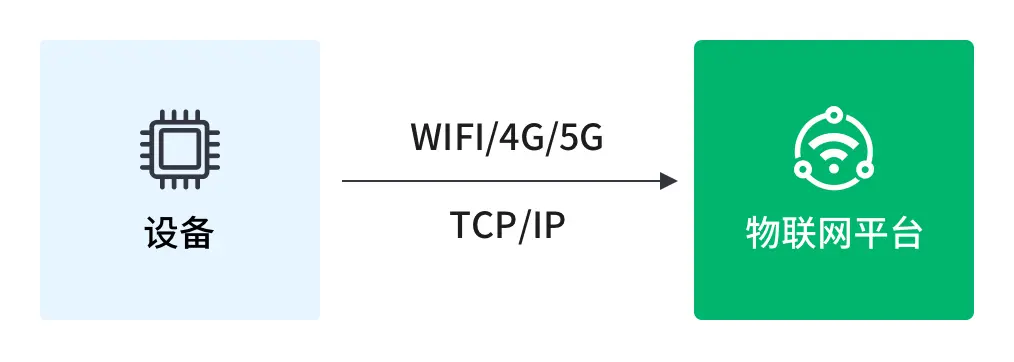
\includegraphics[width=0.8\linewidth]{../design/IoT1.png}
    \caption{IoT1}
    \label{fig:IoT1}
\end{figure}

网关协议是适用于短距通信无法直接上云的协议,比如蓝牙、ZigBee、LoRa 等。此类设备需要接入网关转换之后,通过 TCP/IP 协议进行上云。

\begin{figure}[H]
    \centering
    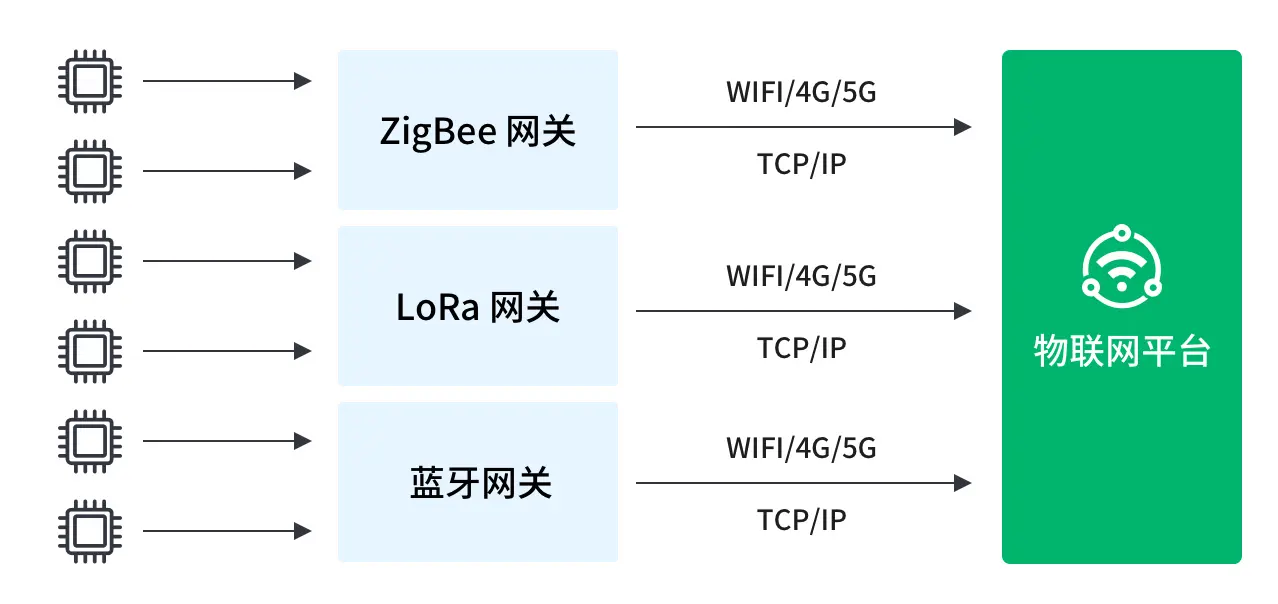
\includegraphics[width=0.8\linewidth]{../design/IoT2.png}
    \caption{IoT2}
    \label{fig:IoT2}
\end{figure}

本系统不考虑网关协议,只考虑应用层协议。系统将支持不同种类的电子秤,支持包含 HTTP、MQTT、MQTT-SN、CoAP、STOMP 在内的多种物联网通信协议。

为了降低开发成本,除了 HTTP、MQTT 这两种通信协议,其它物联网协议采用网关转换的方法来提供支持,网关将对各类协议转换成 MQTT 协议与 MQTT Broker 进行通信,认证规则和消息的持久化规则遵循 MQTT 协议标准。

这里主要分析两种协议:HTTP 和 MQTT。

HTTP(HyperText Transfer Protocol)即超文本传输协议,是一种用于分布式、协作式和超媒体信息系统的应用层协议。在电子秤系统中,通过调用 HTTP 接口上传称重信息具有以下特点:

一、稳定性和通用性:HTTP 是互联网上广泛使用的协议,具有很高的稳定性和通用性。几乎所有的网络设备和软件都支持 HTTP 协议,这使得电子秤可以很容易地与各种不同的系统进行集成。无论是传统的服务器架构,还是现代的云服务平台,都可以通过 HTTP 接口接收电子秤上传的称重信息。例如,许多企业的内部管理系统、电商平台的库存管理系统等都可以通过 HTTP 接口与电子秤进行数据交互,实现实时的库存更新和物流跟踪\cite{Zhao2016}。

二、易于开发和调试:HTTP 协议的开发和调试工具非常丰富。开发人员可以使用常见的编程语言和开发框架,如 Java、Python、Node.js 等,轻松地实现 HTTP 接口的调用和数据处理。同时,各种网络调试工具,如 Postman、Fiddler 等,可以帮助开发人员快速地测试和调试电子秤与服务器之间的通信,确保数据的准确传输。

三、支持多种数据格式:HTTP 协议支持多种数据格式的传输,如 JSON、XML 等。这使得电子秤可以根据不同的应用需求,选择合适的数据格式上传称重信息。例如,对于需要与第三方系统进行数据集成的场景,可以选择使用 JSON 格式,因为 JSON 格式具有简洁、易读、易于解析等优点,被广泛应用于 Web 开发和数据交换领域。

MQTT(Message Queuing Telemetry Transport)即消息队列遥测传输协议,是一种轻量级的发布/订阅模式的消息传输协议。在电子秤系统中,发送 MQTT 消息上传称重信息具有以下优势:

一、低带宽和低功耗:MQTT 协议非常适合在低带宽和低功耗的环境下使用。对于电子秤等物联网设备来说,通常需要在有限的网络资源和电池电量下进行数据传输。MQTT 协议通过采用轻量级的消息格式和高效的发布/订阅模式,可以大大降低网络带宽的占用和设备的功耗。例如,在一些偏远地区或者移动环境下,网络带宽可能非常有限,此时使用 MQTT 协议可以确保电子秤能够及时上传称重信息,同时不会对网络造成过大的负担\cite{Jia2015}。

二、实时性和可靠性:MQTT 协议支持 QoS(Quality of Service)级别,可以根据不同的应用需求,选择不同的消息传输质量级别。在 MQTT 协议中,QoS 有三种级别\cite{Jia2015},分别是:

1、QoS0 – “最多一次”:消息最多传送一次,不保证消息到达目标。适用于实时性要求非常高,但对消息丢失容忍的场景。

2、QoS1 – “至少一次”:保证消息至少传送一次,但可能会重复。适用于需要消息可靠到达,但不介意重复接收的情况。

3、QoS2 – “只有一次”:确保每条消息只会传送一次,且无重复。适用于对消息的唯一性和可靠性有较高要求的场景。

对于需要实时上传称重信息的场景,可以选择 QoS1 或 QoS2 级别,确保消息的可靠传输。同时,MQTT 协议的发布/订阅模式可以实现实时的数据推送,当电子秤上传称重信息后,订阅了该主题的客户端可以立即收到消息,实现实时的数据更新。

三、易于扩展和集成:MQTT 协议具有良好的扩展性和集成性。可以很容易地与其他物联网协议和技术进行集成,如 CoAP、HTTP、WebSocket 等。同时,MQTT 协议的发布/订阅模式可以支持大规模的设备连接和数据传输,适用于构建物联网应用平台。例如,在智慧农业大棚测控系统中,采用 MQTT 协议将智慧大棚测控系统和阿里云物联网平台结合在一起,通过手机 APP 或 PC 软件访问阿里云服务器数据库,实现了移动终端对农业大棚实时监测和控制\cite{Liang2020}。

\section{数据库设计}

本软件数据库设计分为三个阶段:概念模型设计、逻辑模型设计和物理模型设计,下面进行具体阐述。

\subsection{概念模型设计}

农业果实称重云端软件中,可以抽象出七个实体对象,分别是果实、员工、电子秤、采摘作业、称重记录、MQTT客户端、MQTT授权信息,具体分析如下:

1、果实(Fruit):代表农场中的果实,具有编号(ID)属性。

2、员工(Employee):代表农场中的员工,具有编号(ID)属性。

3、电子秤(Electronic Scale):代表用于称重果实的电子秤,具有编号(ID)和密钥(Key)属性。

4、MQTT 客户端(MQTT Client):代表用于连接 MQTT 服务器的客户端,具有编号(ID)和密码(Password)属性。

5、采摘作业(Picking Task):代表员工采摘果实的作业,具有开始时间、结束时间和采摘结果属性。

6、称重记录(Weighing Record):代表电子秤记录的果实重量,具有称重结果和称重时间属性。

7、MQTT 授权信息(MQTT Authorization Info):代表 MQTT 客户端的授权信息,具有权限信息属性。

针对上述对象,根据实际的业务场景,可以得到如下关系:

\begin{table}[H]
\centering
\resizebox{\textwidth}{!}{%
\begin{tabular}{|c|c|c|}
\hline
\textbf{关系名称} & \textbf{关系类型} & \textbf{描述} \\
\hline
果实 - 采摘关系 & 一对多(1:N) & 一个果实可以被多次采摘,与多个采摘作业相关联。 \\
\hline
员工 - 员工称重记录 & 一对多(1:N) & 一个员工可以进行多次称重记录。  \\
\hline
员工 - 采摘作业 & 一对多(1:N) & 一个员工可以执行多个采摘作业。  \\
\hline
电子秤 - 电子秤称重记录 & 一对多(1:N) & 一个电子秤可以记录多个称重记录。  \\
\hline
电子秤 - 称重记录 & 一对多(1:N) & 一个电子秤可以记录多个称重记录。\\
\hline
采摘作业 - 称重记录 & 一对多(1:N) & 一个采摘作业可以产生多个称重记录(例如,在不同时间多次称重)。  \\
\hline
MQTT 客户端 - 设备认证 & 一对一(1:1) & 每个 MQTT 客户端都必须进行设备认证。 \\
\hline
MQTT 客户端 - 设备授权 & 一对多(1:N) & 一个 MQTT 客户端可以拥有多个授权信息。  \\
\hline
员工 - 称重记录 & 一对多(1:N) & 一个员工可以产生多个称重记录。\\
\hline
电子秤 - 设备认证 & 一对一(1:1) & 每个电子秤都必须进行设备认证。  \\
\hline
\end{tabular}%
}
\caption{实体关系及属性表}
\end{table}

将上述分析进行归纳,得到 ER 图如下:

\begin{figure}[H]
    \centering
    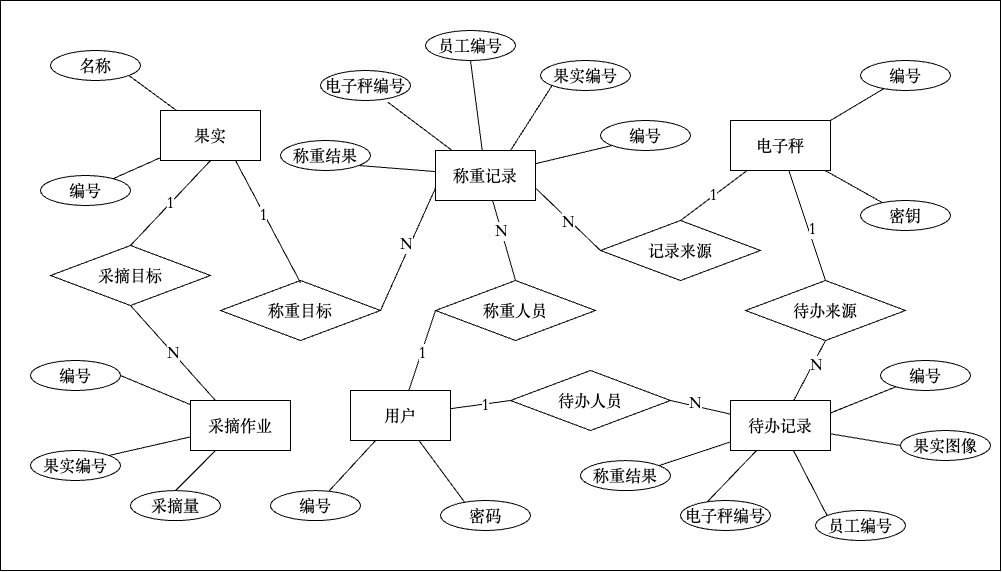
\includegraphics[width=0.8\linewidth]{../design/数据库概念模型设计.png}
    \caption{数据库概念模型设计}
    \label{fig:数据库概念模型设计}
\end{figure}

该 ER 图展示了一个农场管理系统中各个实体之间的复杂关系,包括果实、员工、电子秤和 MQTT 客户端。通过这些关系,系统可以有效地跟踪果实的采摘、称重和授权信息,从而实现高效的农场管理。

\subsection{逻辑模型设计}

本部分详细描述了系统各个表的结构及其字段定义,涵盖了表之间的关系、字段的数据类型及约束条件。每个表的设计都遵循规范化原则,以确保数据的一致性、完整性和高效性。字段的定义包括主键、外键、唯一约束、非空约束等,同时考虑了查询和更新的效率,力求在保证系统扩展性的同时,实现良好的性能表现。

% t_user
\begin{table}[H]
    \centering
    \caption{用户表 (t\_user)}
    \begin{tabular}{|l|l|l|l|}
    \hline
    字段 & 类型 & 约束 & 说明 \\
    \hline
    id & bigint & 主键 & 自增主键 \\
    uid & varchar(255) & 非空,唯一 & 用户认证编号 \\
    name & varchar(255) & 非空 & 用户名称 \\
    password & varchar(255) & 非空 & 密码(加密) \\
    roles & varchar(255) & - & 角色(英文逗号分隔) \\
    create\_time & bigint & 非空 & 创建时间(毫秒级时间戳) \\
    update\_time & bigint & 非空 & 更新时间(毫秒级时间戳) \\
    status & int & 非空 & 状态(0禁用/1启用/2已删除) \\
    \hline
    \end{tabular}
    \end{table}

% t_produce
\begin{table}[H]
\centering
\caption{果实表 (t\_produce)}
\begin{tabular}{|l|l|l|l|}
\hline
字段 & 类型 & 约束 & 说明 \\
\hline
id & bigint & 主键 & 系统自带从0开始,用户添加从1000000开始 \\
name & varchar(255) & 非空,唯一 & 果实名称 \\
name\_en & varchar(255) & 唯一 & 果实英文名称 \\
create\_time & bigint & 非空 & 创建时间(毫秒级时间戳) \\
update\_time & bigint & 非空 & 更新时间(毫秒级时间戳) \\
status & int & 非空 & 状态(0未种植/1在种植/2已删除) \\
\hline
\end{tabular}
\end{table}

% ## t_work
\begin{table}[H]
\centering
\caption{采摘作业表 (t\_work)}
\begin{tabular}{|l|l|l|l|}
\hline
字段 & 类型 & 约束 & 说明 \\
\hline
id & bigint & 主键 & 自增主键 \\
produce\_id & bigint & 非空 & 果实编号 \\
start\_time & bigint & 非空 & 采摘开始时间(毫秒级时间戳) \\
end\_time & bigint & 非空 & 采摘结束时间(毫秒级时间戳) \\
data\_value & decimal(10,2) & - & 总的采摘称重结果 \\
unit & int & - & 称重单位(0mg/1g/2kg/3t/4lb/5oz/6ct) \\
create\_time & bigint & 非空 & 创建时间(毫秒级时间戳) \\
update\_time & bigint & 非空 & 更新时间(毫秒级时间戳) \\
status & int & 非空 & 状态(0未开始/1进行中/2已结束/3已取消/4已删除) \\
\hline
\end{tabular}
\end{table}

% t_scale
\begin{table}[H]
\centering
\caption{电子秤表 (t\_scale)}
\begin{tabular}{|l|l|l|l|}
\hline
字段 & 类型 & 约束 & 说明 \\
\hline
id & bigint & 主键 & 自增主键 \\
sid & varchar(255) & 非空 & MQTT 用户认证编号 \\
model & varchar(255) & - & 型号 \\
max\_capacity & decimal(10,2) & 非空 & 最大量程 \\
min\_capacity & decimal(10,2) & 非空 & 最小量程 \\
unit & int & 非空 & 量程单位(0mg/1g/2kg/3t/4lb/5oz/6ct) \\
verification\_interval & int & - & 检定分度值 \\
display\_interval & int & - & 显示分度值 \\
unit\_dv & int & - & 分度值单位(0mg/1g/2kg/3t/4lb/5oz/6ct) \\
protocol & varchar(255) & - & 协议(小写,逗号分隔) \\
create\_time & bigint & 非空 & 创建时间(毫秒级时间戳) \\
update\_time & bigint & 非空 & 更新时间(毫秒级时间戳) \\
status & int & 非空 & 状态(0禁用/1启用/2已删除) \\
\hline
\end{tabular}
\end{table}

% t_record
\begin{table}[H]
\centering
\caption{称重记录表 (t\_record)}
\begin{tabular}{|l|l|l|l|}
\hline
字段 & 类型 & 约束 & 说明 \\
\hline
id & bigint & 主键 & 自增主键 \\
work\_id & bigint & 非空 & 采摘作业编号 \\
produce\_id & bigint & 非空 & 果实编号 \\
image & varchar(255) & - & 果实图片地址 \\
employee\_id & bigint & 非空 & 员工编号 \\
scale\_id & bigint & 非空 & 电子秤编号 \\
data\_value & decimal(10,2) & 非空 & 称重结果 \\
data\_error\_margin & decimal(10,2) & - & 称量结果误差范围 \\
unit & int & 非空 & 称重单位(0mg/1g/2kg/3t/4lb/5oz/6ct) \\
data\_time & bigint & 非空 & 称重时间(毫秒级时间戳) \\
\hline
\end{tabular}
\end{table}

% t_todo
\begin{table}[H]
\centering
\caption{待处理称重记录表 (t\_todo)}
\begin{tabular}{|l|l|l|l|}
\hline
字段 & 类型 & 约束 & 说明 \\
\hline
id & bigint & 主键 & 自增主键 \\
produce\_id & bigint & - & 果实编号 \\
produce\_name & varchar(255) & - & 果实名称 \\
image & varchar(255) & - & 采摘作业图片地址 \\
employee\_id & bigint & 非空 & 员工编号 \\
scale\_id & bigint & 非空 & 电子秤编号 \\
data\_value & decimal(10,2) & 非空 & 称重结果 \\
data\_error\_margin & decimal(10,2) & - & 称量结果误差范围 \\
unit & int & 非空 & 称重单位(0mg/1g/2kg/3t/4lb/5oz/6ct) \\
data\_time & bigint & 非空 & 称重时间(毫秒级时间戳) \\
\hline
\end{tabular}
\end{table}

% ## t_mqtt_acl
\begin{table}[H]
\centering
\caption{MQTT 访问控制表 (t\_mqtt\_acl)}
\begin{tabular}{|l|l|l|l|}
\hline
字段 & 类型 & 约束 & 说明 \\
\hline
id & int & 主键 & 自增主键 \\
username & varchar(255) & 非空 & MQTT 认证用户名 \\
permission & varchar(255) & 非空 & 操作权限(allow/deny,即允许/拒绝) \\
action & varchar(255) & 非空 & 操作类型(publish/subscribe/all,即发布/订阅/所有) \\
topic & varchar(255) & 非空 & 适用主题 \\
qos & int & - & 消息 QoS 级别(0,1,2) \\
retain & int & - & 是否支持发布保留消息(0否/1是) \\
\hline
\end{tabular}
\end{table}

\subsection{物理模型设计}

本系统使用 MySQL 作为数据库管理系统,采用 InnoDB 存储引擎,事务隔离级别设置为可重复读,以确保数据的一致性和可靠性。在后台应用中,数据库访问通过 JPA (Java Persistence API) 进行实现,简化了数据库操作,提升了代码的可维护性和开发效率。

\section{本章小结}

这些设计模式和架构描述展示了农业果实称重云端软件系统的整体设计和通信流程。通过采用前后端分离的架构,结合 Spring 后端的 MVC 模式与 Vue 前端的 MVVM 模式,系统能够更好地处理数据交互和界面更新。系统架构通过分层设计,使得每一层都具备明确的职责,方便后期的扩展和维护。

在通信协议部分,系统的选择了 HTTP 和 MQTT 两种协议,分别适用于不同的应用场景。HTTP 用于传统的接口交互,而 MQTT 则通过低带宽、高可靠性和实时性的优势,适应了物联网环境中的需求。这两种协议的结合使得系统可以灵活应对不同类型的设备和网络条件。

数据库设计部分,构建了清晰的实体关系,确保了数据的完整性和系统的高效运行。通过一对多的关系设计,系统能够记录和管理员工、电子秤、果实等多个维度的数据,从而支持各种业务场景。

%%%%%%%%%%%%%%%%%%%%%%%%%%%%%%%%

\chapter{软件实现与测试}

\section{系统测试的目的与方法}
\section{测试模型}
\section{测试环境}
\section{主要测试用例}
\section{系统测试结果}
\section{本章小结}
\chapter{总结与展望}

\section{论文工作总结}

本文研究深入调研农业生产活动,应用软件工程相关知识理论,归纳与分析具体需求,利用先进软件技术,设计出合理的系统架构并可开发农业果实称重云端软件,实现高性能且稳定可用的智能化农业数据处理流程、高效且丰富的信息管理功能以及多个维度下数据的可视化。整个过程主要完成的工作如下:

1、进行背景调研和需求分析。调研农业生产活动,分析果实收获和称重入库的具体流程,分析并归纳各项需求,划分功能模块,得到工作分解图,为设计开发工作奠定基础。

2、进行软件系统设计。在需求分析的基础上,选用当下可靠的框架和技术,进行总体架构设计、接口设计、数据库设计、具体业务功能的流程设计等。

3、实现软件各项功能组件。根据设计,对业务功能进行编码实现,完成各个软件模块的联调与集成。

4、部署软件并完成各项测试功能。完成功能测试和性能测试,对测试结果进行理论分析,给出相关结论。

\section{后续工作展望}

TODO: 更详细一点。

1、EMQX 动态集群

2、扩大数据集,训练更好的图像识别模型

\end{document}
